\subsection{Seleção do Número de Clusters: Método do Cotovelo}

A definição do número ideal de clusters ($k$) é uma etapa crucial em experimentos de agrupamento. Neste trabalho, utilizou-se o \textbf{método do cotovelo} aplicado aos dados balanceados e normalizados de cada base para determinar o valor mais adequado de $k$.

Para o conjunto \textbf{Adult}, avaliou-se o comportamento da soma das distâncias quadráticas internas (inertia) para valores de $k$ variando de 2 a 24. Observa-se, na Figura~\ref{fig:elbow_adult}, uma queda acentuada da inércia até $k=8$, caracterizando o "cotovelo" da curva. Esse ponto sugere que oito clusters são suficientes para capturar a estrutura principal dos dados, ainda que o número de classes reais seja dois (<=50K e >50K), indicando a presença de subgrupos relevantes na estrutura dos dados.

No caso do \textbf{Dry Bean}, o mesmo procedimento foi realizado, variando $k$ de 2 a 24. O gráfico apresentado na Figura~\ref{fig:elbow_drybean} evidencia o cotovelo em $k=7$, valor alinhado ao número de cultivares presentes no conjunto, indicando que sete clusters representam adequadamente a diversidade das classes reais.

Assim, o método do cotovelo fundamentou a escolha do número de clusters nos experimentos, garantindo avaliações justas e alinhadas à estrutura dos dados. As Figuras a seguir ilustram o comportamento da inércia em função de $k$ para cada base:

\begin{figure}[ht]
    \centering
    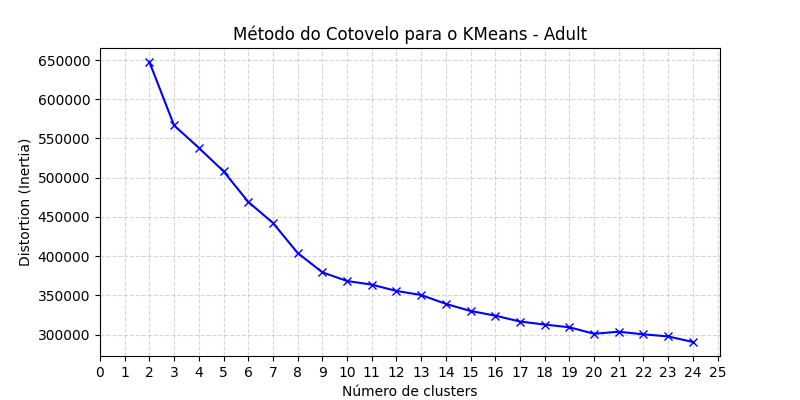
\includegraphics[width=0.8\linewidth]{../src/img/kmeans_adult_elbow.png}
    \caption{Curva do método do cotovelo para o dataset Adult balanceado. O "cotovelo" ocorre em $k=8$.}
    \label{fig:elbow_adult}
\end{figure}

\begin{figure}[ht]
    \centering
    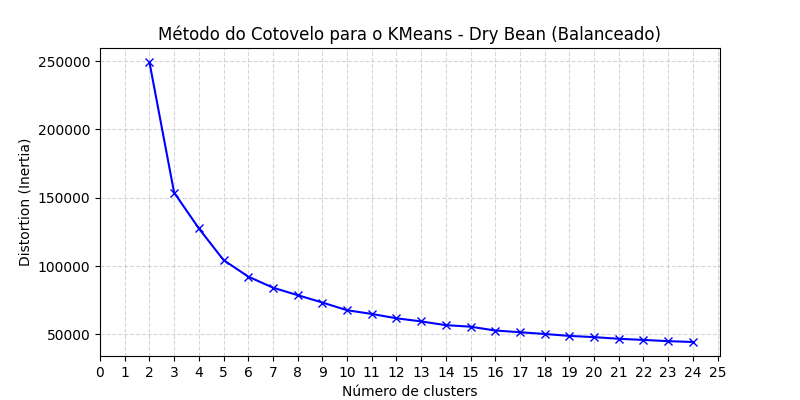
\includegraphics[width=0.8\linewidth]{../src/img/kmeans_drybean_balance_elbow.png}
    \caption{Curva do método do cotovelo para o dataset Dry Bean balanceado. O "cotovelo" ocorre em $k=7$.}
    \label{fig:elbow_drybean}
\end{figure}